\documentclass[tikz, margin=10mm]{standalone}

\usepackage{tikz}

\usetikzlibrary{calc}
\usetikzlibrary{arrows, arrows.meta}

\begin{document}

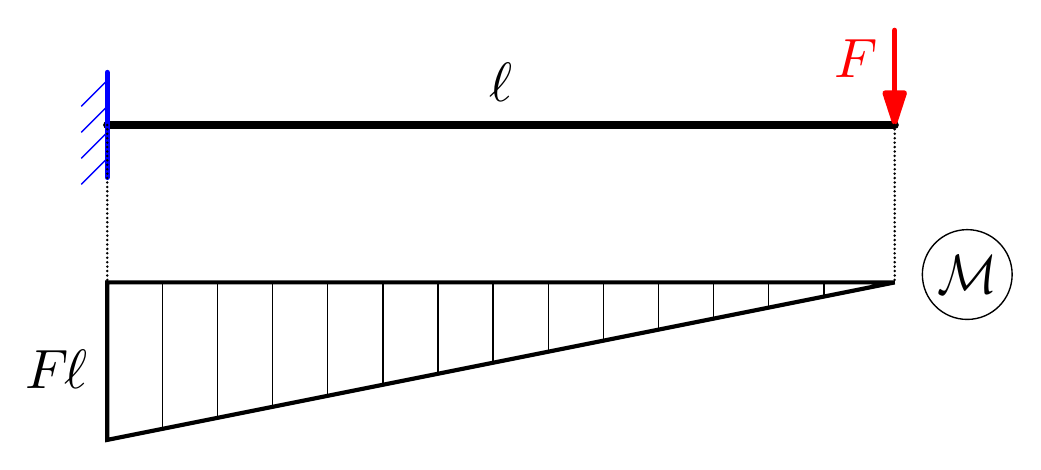
\begin{tikzpicture}[scale=1]

\def\beamlength{10}

% beam

\draw [line width=3pt, line cap=round, color=black]
	(0, 0) -- (\beamlength, 0)
		node [pos=0.5, above, shape=circle, fill=white, inner sep=-2pt, outer sep=10pt] {\scalebox{2}{$\ell$}} ;

% constraints

\def\clamplength{1.33}

\tikzstyle{constraint line} = [line width=2pt, color=blue, line cap=round]
\tikzstyle{constraint hatch} = [line width=.5pt, blue]

\draw [constraint line] (0, 0) -- (0, \clamplength / 2) ;
\draw [constraint line] (0, 0) -- (0, - \clamplength / 2) ;

\def\clamphatchsize{.33}
\pgfmathsetmacro\hatchamplitude{( \clamplength / 2 ) - .1}
\pgfmathsetmacro\hatchstep{.33}
\pgfmathsetmacro\nexthatch{\hatchamplitude - \hatchstep}
\foreach \ycap in {\hatchamplitude, \nexthatch, ..., -\hatchamplitude}
	\draw [constraint hatch] (0, \ycap) -- (-\clamphatchsize, \ycap - \clamphatchsize) ;

% external loads

\tikzstyle{force line} =
	[line width=2pt, red, line cap=round, -{Triangle[round, length=15pt, width=9pt]}]

\draw [force line] (\beamlength, 1.2) -- (\beamlength, 0)
	node [pos=0.7, above left, shape=circle, fill=white, inner sep=-2pt, outer sep=12pt] {\scalebox{2}{$F$}} ;

% epure of bending moments

\def\epurelvl{-2}
\def\maxmoment{2}

\tikzstyle{epure line} = [line width=1.5pt, color=black, line cap=round]
\tikzstyle{epure hatch} = [line width=.5pt, color=black]
\tikzstyle{epure aux} = [line width=1pt, color=black, line cap=round, dash pattern=on 0pt off 1.6\pgflinewidth]

\draw [epure aux] (0, 0) -- (0, \epurelvl) ;
\draw [epure aux] (\beamlength, 0) -- (\beamlength, \epurelvl) ;

\foreach \xhatch in {0, .7, ..., \beamlength}
	\pgfmathsetmacro\currentmoment{\maxmoment * ( 1 - ( \xhatch / \beamlength ) )}
	\draw [epure hatch] (\xhatch, \epurelvl) -- (\xhatch, \epurelvl - \currentmoment) ;

\draw [epure line] (0, \epurelvl) -- (0, \epurelvl - \maxmoment) -- (\beamlength, \epurelvl) -- cycle ;

\draw [epure aux] (0, \epurelvl) -- ++(0, -\maxmoment)
	node [pos=0.55, left, shape=circle, fill=white, inner sep=-2pt, outer sep=8pt]
	{\scalebox{2}{$F\hspace{-0.2ex}\ell$}} ;

\newcommand\internalmoment{\scalebox{.9}[1]{$ \mathcal{M} $}}

\node [right, shape=circle, draw=black, line width=.5pt, fill=white, inner sep=2.5pt, outer sep=10pt]
	at (\beamlength, \epurelvl + .1) {\scalebox{2}{\internalmoment}} ;

\end{tikzpicture}

\end{document}